% !TEX root = ../entropy.tex

\section{Spending profiles predict emergency savings}%
\label{sec:results}

Table~\ref{tab:main} shows the effect of entropy on the
probability of building emergency savings in a given month. Columns (1)-(3)
show results for unsmoothed entropy based on 9 categories, 48 categories, and
merchant names, respectively. Columns (4)-(6) results for smoothed entropy
based on the same variables. All models include user and year-month fixed
effects, and standard errors are clustered at the user-level. 95\% confidence
intervals are shown in brakets.

\begin{table}[ht]
\centering\tiny
\caption{Effect of entropy on P(savings transactions)}
\label{tab:main}
\input{\tabdir/reg_has_inflows_main.tex}
\tabnote{.95\textwidth}{Results from estimating Equation~\ref{equ:model}. The
    dependent variable in all columns is a dummy variable indicating whether a
    user made at least one transaction into any of their savings accounts in a
given period. \regtabinfo}
\end{table}

Results for unsmoothed entropy suggest that a one unit increase in entropy is
associated with an increase in the probability of a user making at least one
transfer into their savings accounts of between 1.1 and 2.3 percentage points
-- an effect up to two times larger than that of a \pounds1000 increase in
monthly income. Conversely, the effect for unsmooth entropy tends to be
somewhat smaller in magnitude but runs in the reverse direction: a one-unit
increase in the smoothed entropy score is associated with a reduction in the
probability of transferring money into savings account of between 0.4 and 1.7
percentage points.

As discussed in Section~\ref{sub:estimation}, these results are not a results
of reverse causality. While we might think that making a savings transactions
might change some or all of the components of entropy discussed in
Section~\ref{sub:spending_profiles} -- the number of unique spending categories
with positive frequency count, the standard deviation of these counts, and the
total number of spend transactions -- and thus change entropy, this is not the
case because of the way we define entropy and savings, and the way spending
transactions are categorised. We define entropy based on all current account
debits that are identified as spends, while we define savings transactions as
the sum of all savings accounts credits. If a user transfers money from their
current account to their savings account, this will be identified as a savings
transaction, but be identified as a transfer on their current account and thus
not considered when calculating their entropy score.

The estimates of our control variables are largely as expected, with the
exception of monthly spend, which one might have expected to be negatively
correlated with savings. Also, it is evident that the strongest predictor among
the included controls for whether a user makes any savings transfer is whether
they receive any income in that month. Income variability, in contrast, is not
correlated with savings behaviour in any economically significant way,
suggesting that people with variable incomes do not build savings cushions for
periods where they have no income.

Overall, the effect of entropy in spending profiles is statistically and
economically significant, and robust across different definitions. In other
words, the scores seem to pick up a feature of the spending distribution that
is predictive of savings behaviour. The obvious question raised by the results
is why smoothing entropy scores flips the direction of the effect of entropy.
We address this next.


\subsection{Why does smoothing flip the direction of the effect}%
\label{sub:why_does_smoothing_flip_the_direction_of_the_effect}

One way to think about the sign change in Table~\ref{tab:main}
is to realise that it implies that at least for some individuals, the relative
rank of smoothed and unsmoothed entropy must differ considerably -- there must
be some individuals that have low unsmoohed entropy but high smoothed entropy
or high unsmoothed entropy and low smoothed entropy or both. Understanding who
those individuals are might thus help us understand the sign flip.

To understand rank differences between unsmoothed and smoothed entropy scores
it is useful to rewrite Equation~\ref{equ:entropy} in a way that makes it easy
to see its component parts. Remember from Section~\ref{sub:spending_profiles}
that $\setc$ is the set of all spending categories, and let $\setcp = \{c: f_c
> 0\}$ be the set of all spending categories with positive frequency counts
(i.e.  with at least one transaction) and $\setcz = \{c: f_c = 0\}$ the set of
all spending categories with a zero frequency count, so that $\setc = \setcz
\cup \setcp$. Remember also that $f_c$ is the frequency count of spending
category $c$ -- the number of transactions user $i$ made in category $c$ in
period $t$ -- and $F$ is the total number of transactions made by that user in
that period. Then, using our definitions of unsmoothed and smoothed
probabilities, we can write unsmoothed entropy as

\begin{equation}
\label{equ:entropy_us}
H = -\sum_{c \in \setcp}{\left(\frac{f_c}{F}\right)
log\left(\frac{f_c}{F}\right)},
\end{equation}

and smoothed entropy as:

\begin{equation}
\label{equ:entropy_s}
H^s = -\sum_{c \in \setcp}{\left(\frac{f_c + 1}{F + |\setc|}\right)
log\left(\frac{f_c + 1}{F + |\setc|}\right)}
- |\setcz|\left(\frac{1}{F + |\setc|}\right)
log\left(\frac{1}{F + |\setc|}\right),
\end{equation}

\noindent where the size of set $\setcz$, $|\setcz|$, is the number of all
spending categories in which a user makes no transactions in a certain period.
These expressions make clear that, by definition, unsmoothed entropy is a
function of frequency counts of categories with positive counts only while
smoothed entropy has two parts: the sum over all additively smoothed frequency
counts of categories with positive counts, plus the same sum for the additively
smoothed probabilities of categories with zero counts, which reduces to a
constant term that is multiplied by the number of categories with a zero count.

The expressions also make transparent the three main components of both types
of entropy that are determined by user behaviour. The first is the number of
spending categories with a non-zero frequency count, $|\setcp|$, which
determines the number of elements summed over in Equation~\ref{equ:entropy_us},
and partitions the categories into either contributing to the sum on the left
hand side of Equation~\ref{equ:entropy_s} or to the constant term on the right
hand side. The latter is the case since, for an exogenously fixed $|\setc|$,
$|\setcz| = |\setc \backslash \setcp|$ -- for a given number of total
categories, the number of categories with a zero frequency count is the
difference between the total number of categories and the number of categories
with a positive frequency count. The second component is the variation of the
frequency counts, $f_c$, which will determine the variation in the
probabilities of a spend accurring in a given category. The third component is
the total number of transactions ($F$). The number of total spending
categories, $|\setc|$, also determines smoothed entropy and, implicitly, also
unsmoothed entropy since it ``scales'' the number of categories with a positive
frequency count, $|\setcp|$, as a given number of spending transactions are
categorised into finer or coarser categories. But it is exogenously given and
does not depend on user behaviour.

One starting point for thinking about why unsmoothed and smoothed entropy
differ is thus to think about how these three components effect the two scores
differently. From equations~\ref{equ:entropy_us} and~\ref{equ:entropy_s} we can
see that the first part of smoothed entropy that sums over all spending
categories with positive frequency counts is very similar to the entire
expression of unsmoothed entropy -- it is that same expression but with
additively smoothed probabilities. Hence, all else equal, the higher the number
of categories with positive counts, the more smoothed entropy is determined by
that first part, and the more similar it will be to unsmoothed entropy. As a
result, we would expect to find large (rank) differences between entropy scores
among cases with few positive-counts categories.

Next, remember from Section~\ref{sub:spending_profiles} that entropy is higher
the more equal the spending category probabilities are. Hence, for a given
number of zero-count categories, smoothed entropy will be higher if the
(additively smoothed) probabilities of all positive-count categories are close
to the (additively smoothed) probabilities of the zero-count categories, which
will be the case (i) if there are few overall transactions, such that counts
frequency counts ($f_c$) are close to zero and (ii) if there is little
variation in the counts.

\begin{figure}[ht]
    \centering 
    \caption{Effect of smoothing on entropy}
    \label{fig:scatter_facets}
    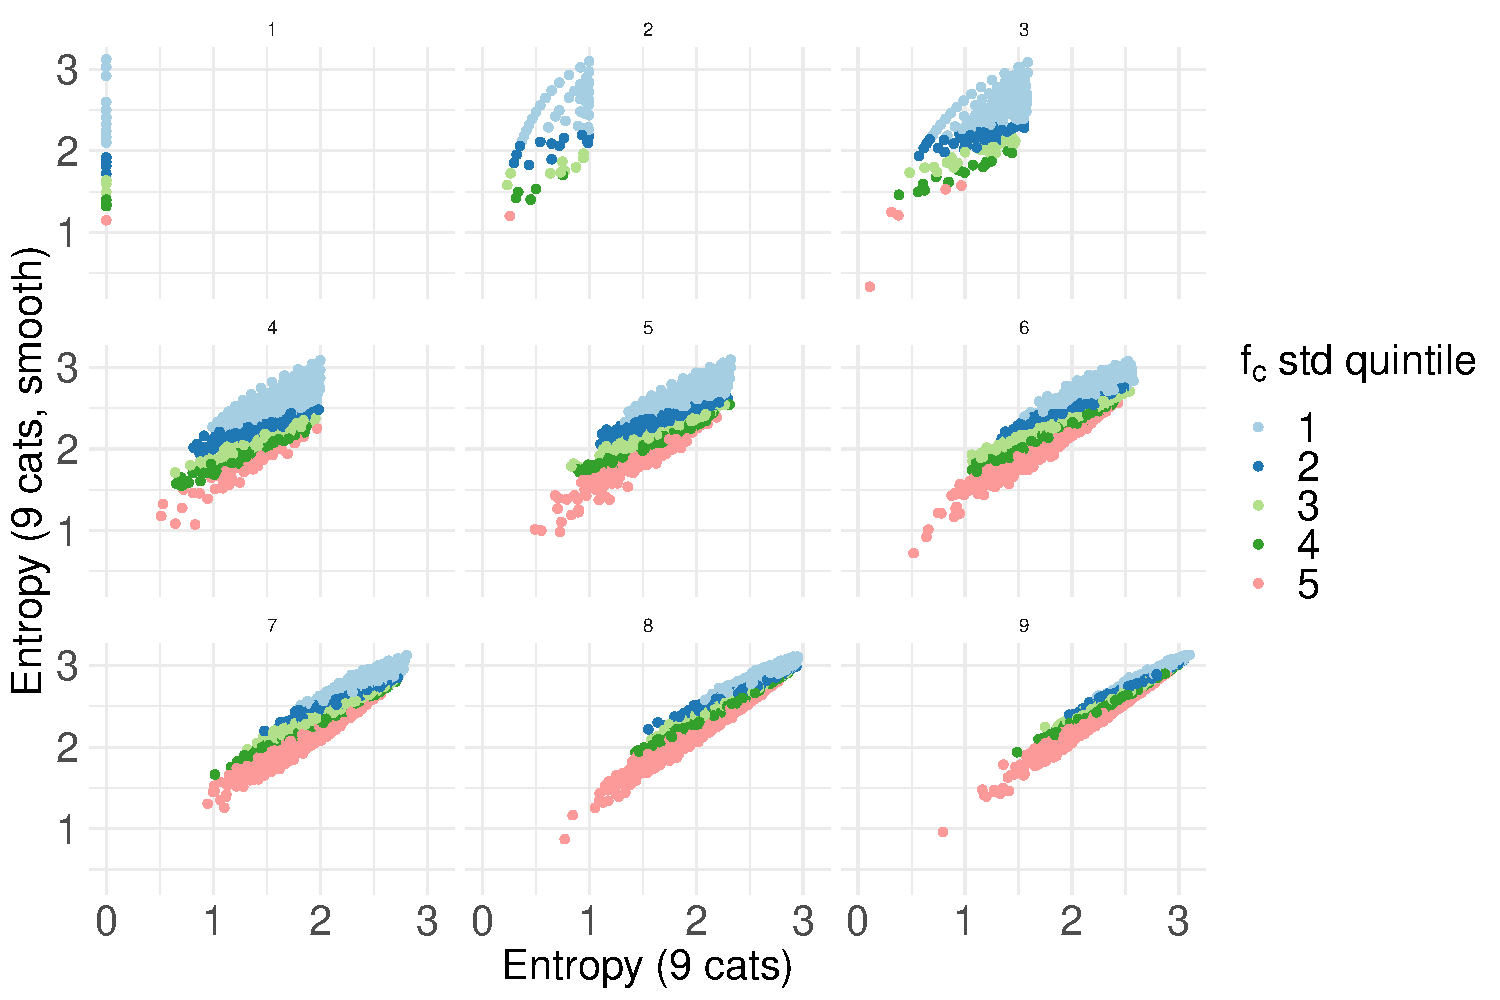
\includegraphics[width=\textwidth]{\figdir/scatter_facet_std_tag_q.pdf}
    \fignote{\textwidth}{Percentile ranks of 9-category-based unsmoothed and
    smoothed entropy separated by the number of categories with positive
frequency counts. White reference lines indicate equal percentile ranks.
Colours indicate frequency count standard deviation quintiles.}
\end{figure}

Figure~\ref{fig:scatter_facets} visualises this intuition for our 9-category
based entropy variable: it shows scatterplots of the percentile ranks of
unsmoothed and smoothed entropy with a reference line indicating identical
rank, separated by the number of categories with positive frequency counts and
coloured based on the quintile of the frequency count standard
deviation.\footnote{Figure~\ref{fig:scatter_facets_txns_count_spend_q} in
    Appendix~\ref{sec:additional_results} a similar plot with colouring based on the
quintile of the total number of transactions. The result is very similar, which
is why we do not show it here.} First, ignoring the colouring and focusing on
the shape of the dots only we can see that, as expected, the relationship
between the two entropy measures is tighter the higher the number of non-zero
spending categories is. Cases with large entropy rank differences are thus to
be found among cases with fewer positive spend categories. Among these, the
colouring makes clear that, as expected, the cases with the largest rank
differences -- those with the furthest vertical difference to the reference
line -- have low variation in their frequency counts. However, it is also clear
that the reverse is not true: there are cases with low frequency variation that
experience little or even a negative rank difference. Hence, while counts
variation is some help in identifying cases with high entropy rank differences,
it does not do so perfectly.

A different way to investigate whether the sign flip can be explained by the
three components of the entropy formula is to test whether entropy captures
anything about users' spending distribution that is predictive of savings
behaviour beyond the information already contained in its three components. If
this is were not the case, then we should be able to explain the sign flip
solely based on the components.

\begin{table}[ht]
\centering\tiny
\caption{Entorpy on components}
\label{tab:entropy_on_components}
\input{\tabdir/reg_entropy_on_components.tex}
\tabnote{.95\textwidth}{\regtabinfo}
\end{table}

As a first step, Table~\ref{tab:entropy_on_components} shows results from
regressing the unsmoothed and smoothed versions of both the 9-category and
48-category based entropy variables on the three components. The components
explain about 75\% of the variation in the 9-category-based and 95\% of the
48-category-based variable. The directions of the effects are consistent across
the two entropy variables as well as accross smoothed and unsmoothed versions
and are as expected: an increase in the number of categories with a positive
frequency count increases entropy (more elements are summed over in
Equation~\ref{equ:entropy_us} and more elements are part of the first part of
the expression in Equation~\ref{equ:entropy_s}), a higher variation in
spend category frequency counts reduces entropy (the uniform distribution is
the maximum entropy distribution), and the total number of spending
transactions increases entropy.\footnote{The direction of the relationship between the number of
total spend transaction and entropy is less obvious than that of the other two
components. Taking the derivative of Equation~\ref{equ:entropy_us} with respect
to $F$ shows that the relationship is guaranteed to be positive if the
frequency count of each category is less than $F/2$.}

Next, we look at whether the relationship between spending entropy and the
probability of making a savings transaction remains economically and
statistically significant once we control for the three components. Columns (1)
and (3) in Table~\ref{tab:main} replicate the results for the 48-category-based
unsmoothed and smoothed entropy measures presented in Table~\ref{tab:main} for
reference. In columns (2) and (4) we additionally control for the three entropy
components. Including these components has some effect: the coefficients change
slightly -- decreasing in absolute magnitude in the case of unsmoothed entropy,
increasing in the case of smoothed entorpy -- while the width of the confidence
intervals about double in both cases, reflecting the strong collinearity amont
the component and entropy. However, both coefficients remain statistically
significant and their confidence intervals cover values that are also
economically significant. Hence, the results make clear that the results in
Table~\ref{tab:main} cannot be attributed simply to the effect of one or more
of entropy's simple components.

\begin{landscape}
\begin{table}[ht]
\centering\footnotesize
\caption{Controlling for components}
\label{tab:components}

\begin{table}[htbp]
   \centering
   \tiny
   \begin{threeparttable}[b]
      \caption{\label{tab:reg_has_inflows_comp} Controlling for entropy components}
      \begin{tabular}{lcccc}
         \tabularnewline \midrule \midrule
         Model:                    & (1)             & (2)             & (3)              & (4)\\  
         \midrule
         \emph{Variables}\\
         Entropy (48 cats)         & 0.029$^{***}$   & 0.013$^{***}$   &                  &   \\   
                                   & [0.025; 0.033]  & [0.006; 0.021]  &                  &   \\   
         Entropy (48 cats, smooth) &                 &                 & -0.023$^{***}$   & -0.028$^{***}$\\   
                                   &                 &                 & [-0.025; -0.020] & [-0.034; -0.022]\\   
         Unique categories         &                 & 0.004$^{***}$   &                  & 0.004$^{***}$\\   
                                   &                 & [0.003; 0.005]  &                  & [0.004; 0.005]\\   
         Category counts std.      &                 & 0.002           &                  & -0.015$^{***}$\\   
                                   &                 & [-0.001; 0.006] &                  & [-0.018; -0.011]\\   
         Number of spend txns      &                 & 0.000$^{***}$   &                  & 0.001$^{***}$\\   
                                   &                 & [0.000; 0.001]  &                  & [0.001; 0.001]\\   
         Month spend               & 0.009$^{***}$   & 0.005$^{***}$   & 0.008$^{***}$    & 0.005$^{***}$\\   
                                   & [0.008; 0.009]  & [0.004; 0.006]  & [0.007; 0.009]   & [0.005; 0.006]\\   
         Month income              & 0.012$^{***}$   & 0.011$^{***}$   & 0.011$^{***}$    & 0.011$^{***}$\\   
                                   & [0.011; 0.013]  & [0.010; 0.012]  & [0.011; 0.012]   & [0.010; 0.012]\\   
         Has income in month       & 0.084$^{***}$   & 0.079$^{***}$   & 0.085$^{***}$    & 0.078$^{***}$\\   
                                   & [0.075; 0.092]  & [0.070; 0.087]  & [0.076; 0.093]   & [0.070; 0.087]\\   
         Income variability        & 0.001$^{*}$     & 0.000           & 0.001$^{*}$      & 0.000\\   
                                   & [-0.000; 0.001] & [-0.000; 0.001] & [-0.000; 0.001]  & [-0.000; 0.001]\\   
         \midrule
         \emph{Fixed-effects}\\
         User                      & Yes             & Yes             & Yes              & Yes\\  
         Year-month                & Yes             & Yes             & Yes              & Yes\\  
         \midrule
         \emph{Fit statistics}\\
         Observations              & 1,043,727       & 1,043,727       & 1,043,727        & 1,043,727\\  
         R$^2$                     & 0.45395         & 0.45498         & 0.45415          & 0.45515\\  
         Within R$^2$              & 0.00768         & 0.00956         & 0.00805          & 0.00986\\  
         \midrule \midrule
         \multicolumn{5}{l}{\emph{Clustered (User) co-variance matrix, 95\% confidence intervals in brackets}}\\
         \multicolumn{5}{l}{\emph{Signif. Codes: ***: 0.01, **: 0.05, *: 0.1}}\\
      \end{tabular}
   \end{threeparttable}
\end{table}



\tabnote{.95\textwidth}{\regtabinfo}
\end{table}
\end{landscape}

